\section{Visuelles System}
Das visuelle System dient zur Verarbeitung visueller Information und umfasst das Auge, den Sehnerv, sowie Teile des Gehirns.

\subsection{Das Auge}
Das Auge ähnelt in seiner Funktion einer Kamera. Die Linse sammelt, unterstützt von der Hornhaut, Lichtstrahlen und projiziert diese als auf dem Kopf stehendes gespiegeltes Bild auf die Netzhaut.
% TODO: Besseres Bild?
\begin{figure}
	\centering
	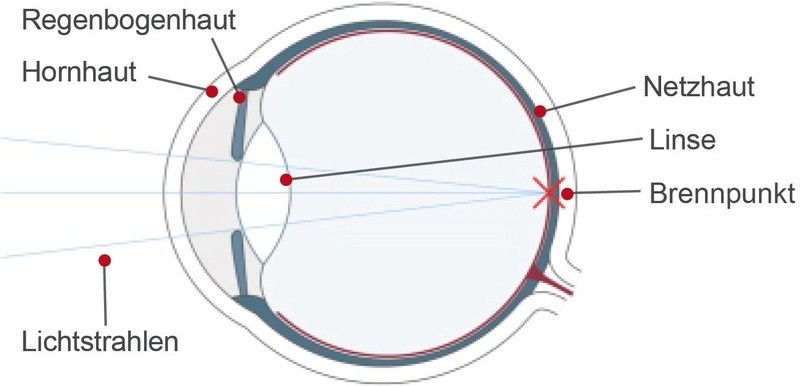
\includegraphics[width=7cm]{images/auge.jpg}
	\caption{Das Auge \cite{auge}}
\end{figure}